\documentclass[xcolor=dvipsnames]{beamer}

\usepackage[font=scriptsize,labelfont=bf]{caption}
\usepackage{url}
\usepackage{hyperref}
\usepackage{verb atim}
\usepackage{amsmath}
\usepackage{graphicx}
\usepackage{ragged2e}
\usepackage{tcolorbox}
\usepackage[dvipsnames]{xcolor}
\usepackage{ulem}
\usepackage{adjustbox}
\usepackage{subcaption}

\usepackage{xcolor}
\usepackage{listings}

% Definir colores
\definecolor{codegreen}{rgb}{0,0.6,0}
\definecolor{codegray}{rgb}{0.5,0.5,0.5}
\definecolor{codeblue}{rgb}{0,0,1}
\definecolor{backcolour}{rgb}{0.95,0.95,0.92}

% Configuración de lstlisting
\lstdefinestyle{mystyle}{
    backgroundcolor=\color{backcolour},   
    commentstyle=\color{codegreen},
    keywordstyle=\color{codeblue}\bfseries,
    numberstyle=\tiny\color{codegray},
    stringstyle=\color{red},
    basicstyle=\ttfamily\footnotesize,
    breakatwhitespace=false,         
    breaklines=true,                 
    captionpos=b,                    
    keepspaces=true,                 
    % numbers=left,                    
    numbersep=5pt,                  
    showspaces=false,                
    showstringspaces=false,
    showtabs=false,                  
    tabsize=2,
    literate={-}{{-}}1 {~}{{\textasciitilde}}1  % Corrige guiones y tildes
}
\lstset{style=mystyle}

\usetheme{Madrid}
%\useoutertheme[subsection=false]{smoothbars}

\AtBeginSection[]{
  \begin{frame}
  \vfill
  \centering
  \begin{beamercolorbox}[sep=8pt,center,shadow=true,rounded=true]{title}
    \usebeamerfont{title}\secname\par%
  \end{beamercolorbox}
  \vfill
  \end{frame}
}

\DeclareMathOperator*{\concat}{\mathbin\Vert}

\definecolor{UBCblue}{rgb}{0.04706, 0.13725, 0.26667} % UBC Blue (primary)
\definecolor{UBCgrey}{rgb}{0.3686, 0.5255, 0.6235} % UBC Grey (secondary)

\setbeamercolor{palette primary}{bg=UBCblue,fg=white}
\setbeamercolor{palette secondary}{bg=UBCblue,fg=white}
\setbeamercolor{palette tertiary}{bg=UBCblue,fg=white}
\setbeamercolor{palette quaternary}{bg=UBCblue,fg=white}
\setbeamercolor{structure}{fg=UBCblue} % itemize, enumerate, etc
\setbeamercolor{section in toc}{fg=UBCblue} % TOC sections
\renewcommand{\figurename}{Fig.}
%\logo{\includegraphics[height=1.2cm]{img/logo_di_black.png}}

% Override palette coloring with secondary
\setbeamercolor{subsection in head/foot}{bg=UBCgrey,fg=white}

\title[Introducción a la Ciencia de Datos - T1]{Análisis Exploratorio de Datos}
\date{2025-03-14}
\author[CNF]{Camilo Esteban Núñez Fernández}
\institute[DI UTFSM]{INF396 - Introducción a la Ciencia de Datos\\ Departamento de Informática}

\begin{document}
	\begingroup 
        \setbeamertemplate{headline}{}
        \begin{frame}
            \titlepage
        \end{frame}
    \endgroup

    \section{Fast Intro}
    \begin{frame}{I.I~$\rhd$~EDA: Exploratory Data Analysis}
    \begin{columns}
        \column{0.5\textwidth}
            \textbf{John Wilder Tukey}
            \begin{figure}
            \centering
            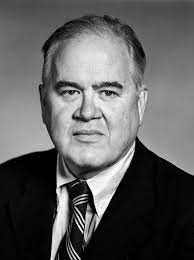
\includegraphics[width=0.5\textwidth]{imgs/intro/portrait.jpeg}
            \end{figure}
            \vspace{3mm}
            \begin{itemize}
                \item Boxplots, Fast Fourier Transform (FFT), Cooley–Tukey FFT algorithm ...
            \end{itemize}
        \column{0.5\textwidth}
            %\pause
            \begin{itemize}
                \item \scriptsize{Exploratory Data Analysis. 1977. Addison-Wesley}
                \begin{figure}
                \centering
                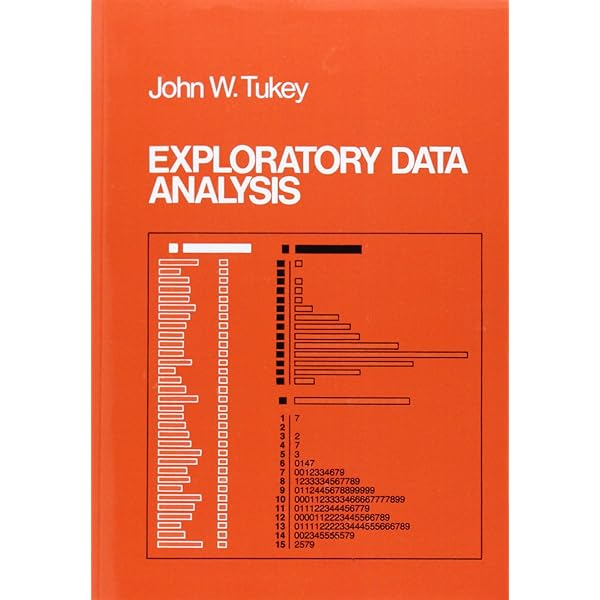
\includegraphics[width=0.4\textwidth]{imgs/intro/book2.jpg}
                \end{figure}
                \item \scriptsize{Data Analysis and Regression: A Second Course in Statistics. 1977 (+ Frederick Mosteller). Addison-Wesley.}
                \begin{figure}
                \centering
                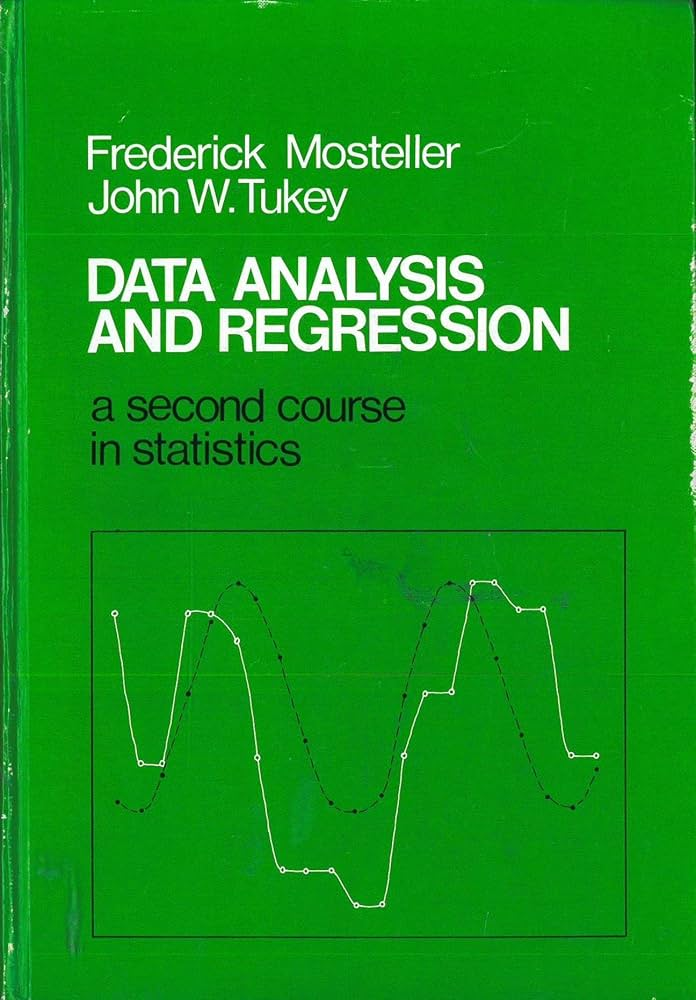
\includegraphics[width=0.3\textwidth]{imgs/intro/book1.jpg}
                \end{figure}
            \end{itemize}
    \end{columns}    
    \end{frame}

    \begin{frame}{I.I~$\rhd$~EDA: Exploratory Data Analysis}
        \begin{itemize}
            \item El Análisis Exploratorio de Datos es un enfoque que emplea diversas técnicas para:
            \vspace{2mm}
            \begin{itemize}
                \item Maximizar la comprensión de un conjunto de datos
                \item Extraer variables importantes
                \item Detectar valores outliers y anomalías
                \item Verificar supuestos subyacentes
                \item Determinar configuraciones óptimas de factores para modelar los datos
            \end{itemize}
            \vspace{2mm}
            \item La mayoría de las técnicas aplicadas en EDA son gráficas, con ciertas técnicas cuantitativas.
        \end{itemize}
    \end{frame}

    \begin{frame}{I.I~$\rhd$~EDA: Exploratory Data Analysis}
        \textbf{¿En qué se diferencia de otros análisis estadísticos?}
        \vspace{3mm}
        \begin{itemize}
            \item Tres enfoques principales: (I) Clásico, (II) Bayesiano, (III) Exploratorio (EDA)
            \vspace{2mm}
            %\pause
            \item \textbf{Clásico}: Asume un modelo a priori. Flujo: Problema~$\rightarrow$~Datos~$\rightarrow$~Modelo~$\rightarrow$~Análisis~$\rightarrow$~Conclusiones
            %\pause
            \item \textbf{Bayesiano}: Incorpora conocimiento experto (prior). Flujo: Problema~$\rightarrow$~Datos~$\rightarrow$~Modelo~$\rightarrow$~Prior~$\rightarrow$~Análisis~$\rightarrow$~Conclusiones
            %\pause
            \item \textbf{Exploratorio (EDA)}: Análisis sin modelo previo para determinar el modelo adecuado. Flujo: \textcolor{DarkOrchid}{Problema~$\rightarrow$~Datos~$\rightarrow$~Análisis~$\rightarrow$~Modelo~$\rightarrow$~Conclusiones}
        \end{itemize} 
    \end{frame}

    \section{Por donde comenzar?}
    \begin{frame}{I.II~$\rhd$~Por donde comenzar?}
        \begin{block}{Formula tus preguntas o requisitos !}
        \begin{itemize}
            \item Útil para guiar el proceso exploratorio.
            \item Útil para reducir el espacio de búsqueda.
            \item Acota tus caminos de exploración.
        \end{itemize}
        \end{block}
        %\pause
        \vspace{5mm}
        \textit{Preguntas sencillas y concisas pueden darte una rápida reducción en la dimensionalidad de los datos !}     
    \end{frame}

    \begin{frame}{I.II~$\rhd$~Formulación de preguntas}
    \begin{figure}
        \centering
        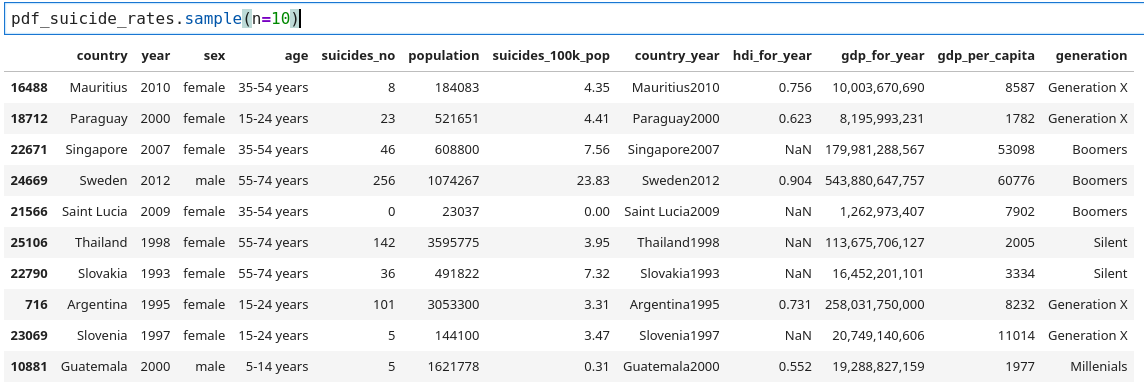
\includegraphics[width=1\linewidth]{imgs/t1_img1.png}
    \end{figure}
    \vspace{2mm}
    \begin{itemize}
        %\pause
        \item Iteración 0: ¿Es la tasa de suicidios mayor en América del Sur que en América del Norte?
        %\pause
        \item Iteración 1: ¿Es la tasa de suicidios por cada 100K hab. mayor en USA que en Chile para la década del 2000?
    \end{itemize}
    \end{frame}

    \section{Estadística Descriptiva}
    \begin{frame}{II~$\rhd$~Estadística Descriptiva}
        \begin{itemize}
            \item Busca \textcolor{DarkOrchid}{resumir y describir características} importantes en los datos. %JungleGreen
            \vspace{2mm}%\pause
            \item Podemos encontrar dos representaciones clásicas:
            \vspace{2mm}%\pause
            \begin{enumerate}
                \item \textbf{Representaciones Numéricas}: Medidas de tendencias y dispersión.
                \vspace{2mm}%\pause
                \item \textbf{Representaciones Gráficas}: Histogramas, Scatter plots, Boxplots, etc.
            \end{enumerate}
        \end{itemize}
    \end{frame}

    \begin{frame}{II.I~$\rhd$~Estadística Descriptiva - Rep. Numéricas}
        %\pause
        \begin{block}{Medidas de Tendencias}
            \begin{itemize}
                \item \textit{Moda}
                \item \textit{Media Muestral}
                \item \textit{Mediana Muestral}
            \end{itemize}
        \end{block}
        \vspace{2mm}%\pause
        \begin{block}{Medidas de Dispersión}
            \begin{itemize}
                \item \textit{Rango}
                \item \textit{Indice de Variación}
                \item \textit{Varianza Muestral}
                \item \textit{Desviación Estándar Muestral}
            \end{itemize}
        \end{block}
        \vspace{2mm}%\pause
        \begin{itemize}
            \item \textbf{Five-Number Summary}: Clásico reporte cuantitativo que incluye, $Q_{1}$ (percentil 25), $Q_{2}$ (percentil 50, mediana), $Q_{3}$ (percentil 75), máximo, mínimo.
        \end{itemize}
    \end{frame}

    \begin{frame}{II.I~$\rhd$~Estadística Descriptiva - Rep. Numéricas}
        \begin{block}{Nota sobre la Desviación Estándar ($\sigma$)}
            \begin{itemize}
                %\pause
                \item $\sigma$ mide la dispersión alrededor de la \textbf{media}($\mu$), por lo que solo debe usarse cuando la media sea la medida de tendencia central elegida.
                %\pause
                \item Si $\sigma=0$ \textbf{solo}, entonces no hay dispersión (todas las observaciones tienen el mismo valor).
                %\pause
                \item Tanto la varianza como la desviación estándar tienen \textbf{buena escalabilidad} en bases de datos grandes.
                % \item Es poco probable que una observación esté a más de varias desviaciones estándar de la media. Según la \textbf{desigualdad de Chebyshev}, al menos $\left(1 - \frac{1}{k^2}\right) \times 100\%$ de las observaciones se encuentran dentro de $k$ desviaciones estándar de la media.
            \end{itemize}
            \vspace{3mm}
            Por estas propiedades, $\sigma$ es un indicador confiable de la dispersión de un conjunto de datos. (Ej. clásico: Análisis de varianza (ANOVA))
        \end{block}
    \end{frame}

    \begin{frame}{II.I~$\rhd$~Estadística Descriptiva - Rep. Numéricas}
        \begin{columns}
            \column{0.5\textwidth}
                \begin{figure}
                \centering
                
\includegraphics[width=0.7\textwidth]{imgs/logos/skimpy_logo.png}
                \end{figure}
            \column{0.5\textwidth}
                \begin{figure}
                \centering
                
\includegraphics[width=0.7\textwidth]{imgs/logos/statsmodels-logo-v2.png}
                \end{figure}
        \end{columns}
    \end{frame}

    \begin{frame}{II.I~$\rhd$~Estadística Descriptiva - Rep. Numéricas}
        \begin{figure}
            \centering
            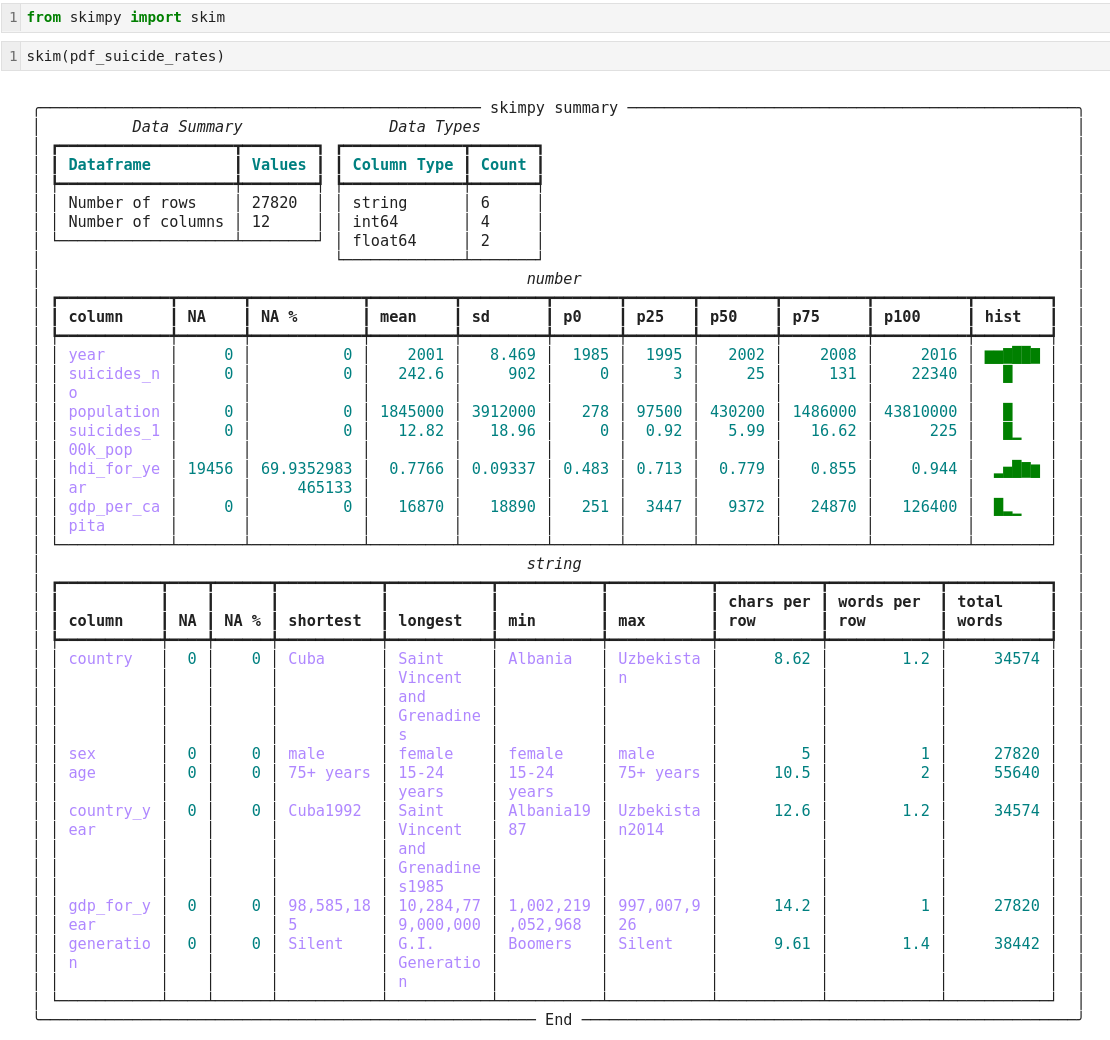
\includegraphics[width=0.7\linewidth]{imgs/t1_img2.png}
        \end{figure}
    \end{frame}

    \begin{frame}{II.I~$\rhd$~Estadística Descriptiva - Rep. Numéricas}
        \begin{figure}
            \centering
            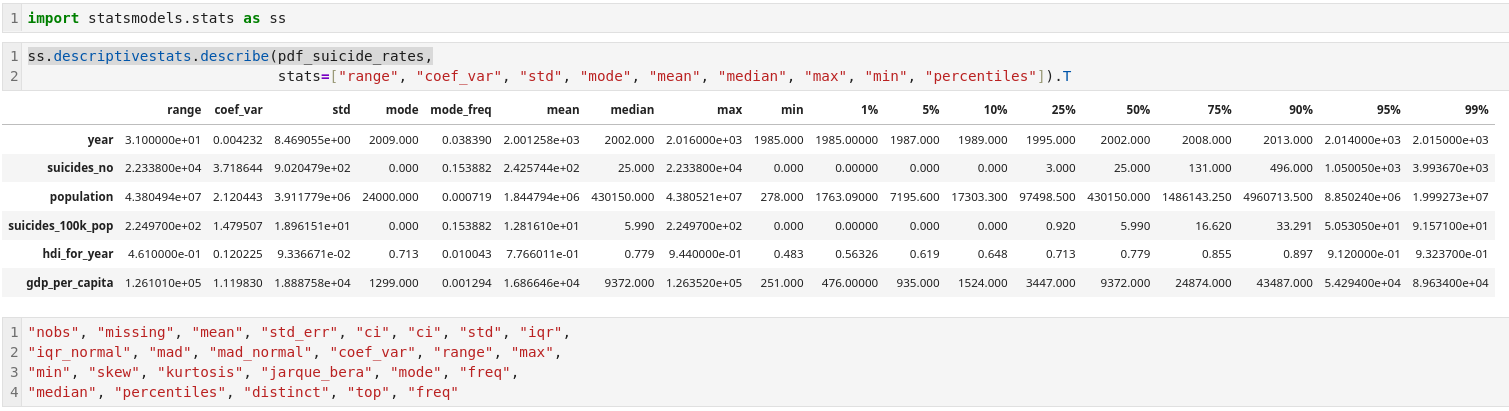
\includegraphics[width=\linewidth]{imgs/t1_img3.png}
        \end{figure}
    \end{frame}

    \begin{frame}{II.I~$\rhd$~Estadística Descriptiva - Rep. Numéricas}
        \begin{figure}
            \centering
            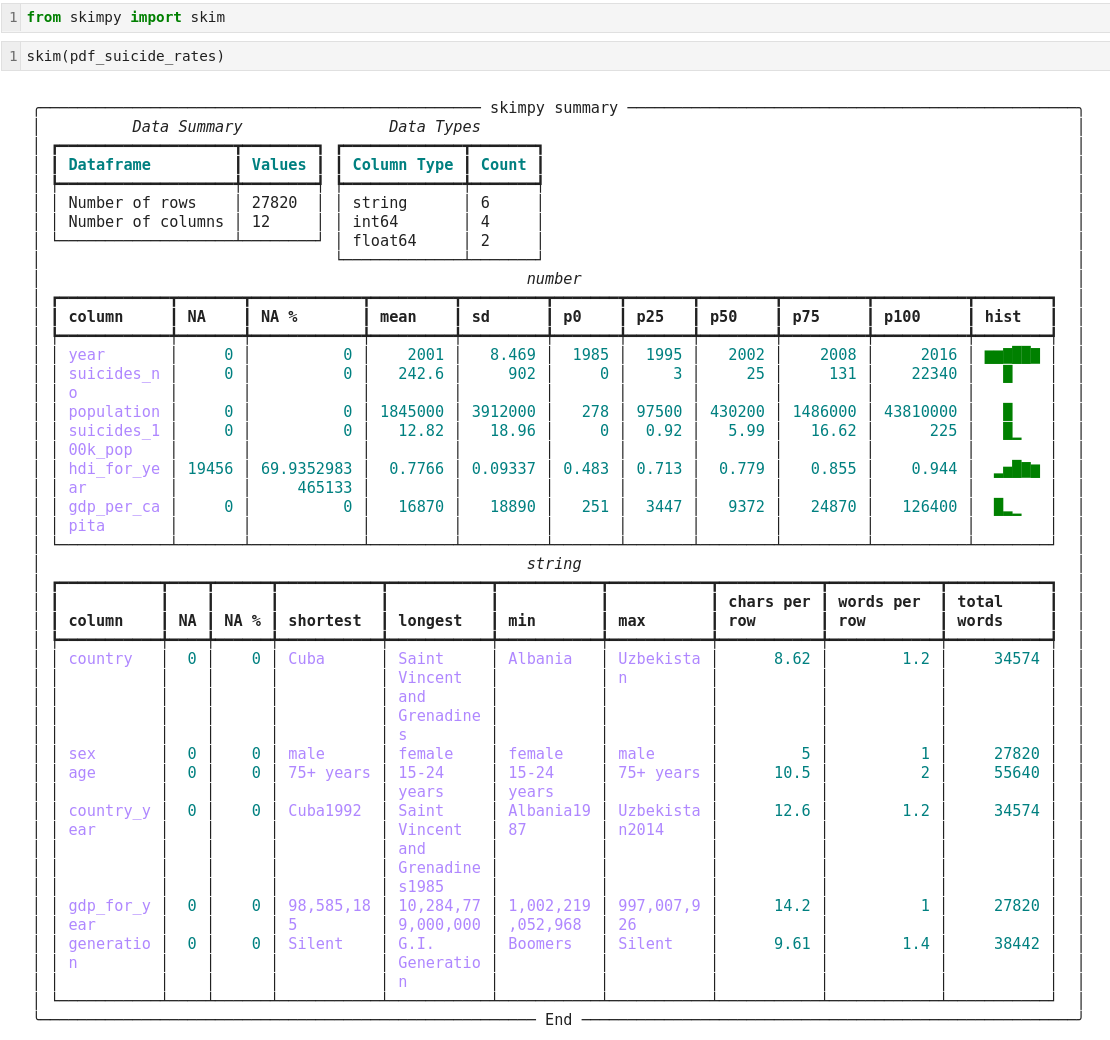
\includegraphics[width=0.7\linewidth]{imgs/t1_img2.png}
        \end{figure}
    \end{frame}

    \begin{frame}{II.II~$\rhd$~Estadística Descriptiva - Rep. Gráficas}
        \begin{block}{¡Considera lo siguiente!}
            \begin{itemize}
                %\pause
                \item Visualizar tus datos mediante gráficos puede facilitar la \textcolor{DarkOrchid}{comprensión de sus propiedades}, la \textcolor{DarkOrchid}{detección de patrones} y la identificación de estrategias de modelado adecuadas para responder a tus preguntas.
                %\pause
                \item Los gráficos también pueden servir como una herramienta de depuración (*debugging*) para validar tu análisis descriptivo.
                %\pause
                \item Es importante diferenciar un gráfico exploratorio de un gráfico final. Los gráficos exploratorios ayudan a inspeccionar los datos en las primeras etapas del análisis, mientras que los gráficos finales están diseñados para comunicar claramente los resultados.
                %\pause
                \item En un gráfico final, prioriza la claridad y la precisión en la comunicación de tus hallazgos.
            \end{itemize}
        \end{block}
    \end{frame}

    \begin{frame}{II.II~$\rhd$~Estadística Descriptiva - Visualización: Barplot}
        \begin{itemize}
            \item Representa la \textcolor{DarkOrchid}{frecuencia} de las \textcolor{DarkOrchid}{categorías} en un conjunto de datos.
            \item Ideal para visualizar datos categóricos y comparar distribuciones.
            \item Se puede usar tanto para conteo directo como para representar valores agregados (por ejemplo, ventas promedio por categoría).
            \item La altura de cada barra refleja la cantidad o proporción de cada categoría.
        \end{itemize}
        \vspace{5mm}
        \begin{figure}
            \centering
            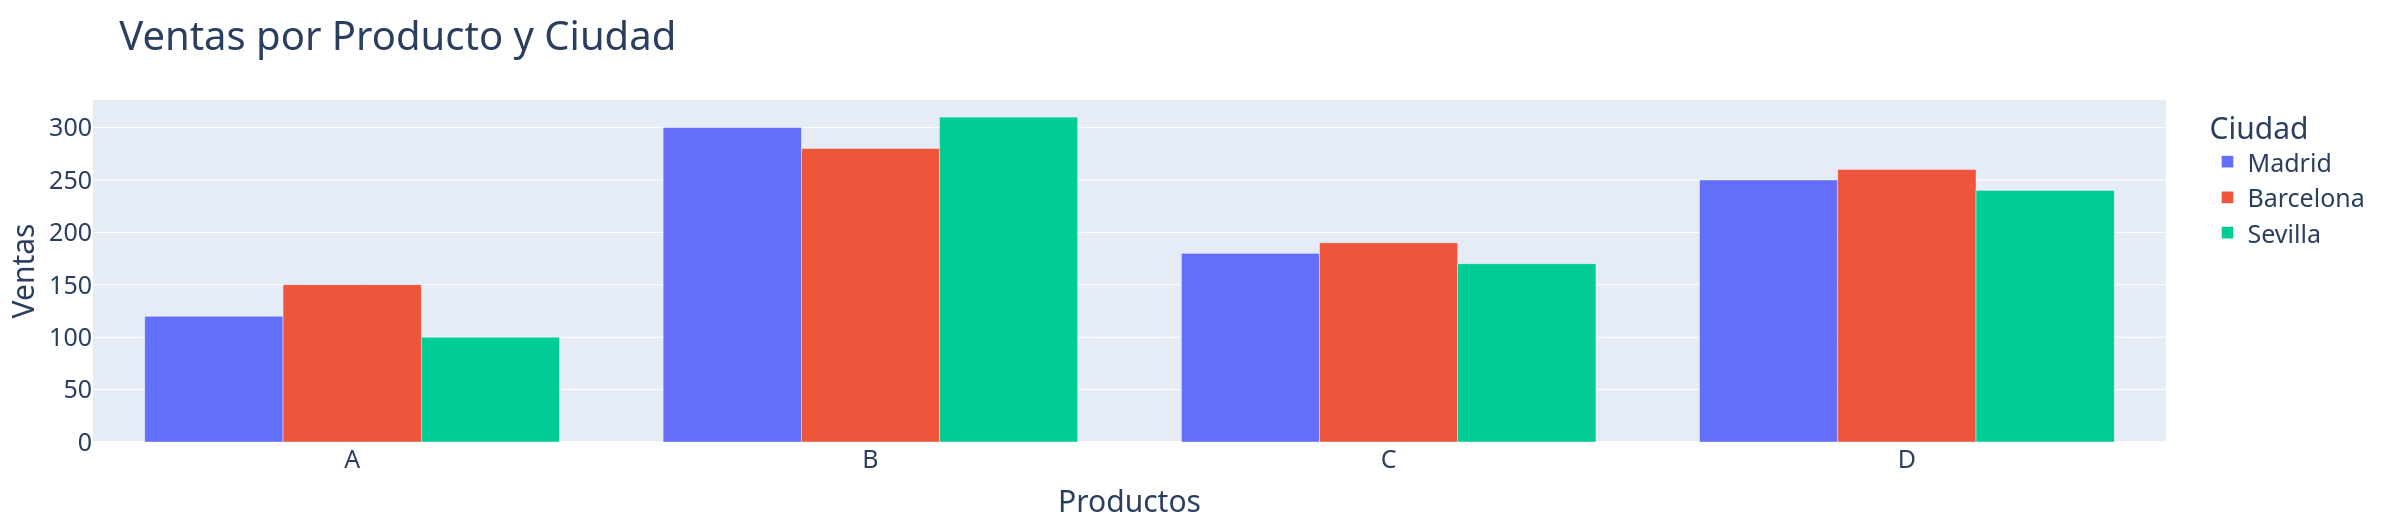
\includegraphics[width=1\linewidth]{imgs/plots/barplot_01.png}
        \end{figure}
    \end{frame}

    \begin{frame}{II.II~$\rhd$~Estadística Descriptiva - Visualización: Histograma}
        \begin{itemize}
            \item Muestra la distribución empírica de todos los datos del conjunto.
            \item Nos ayuda a identificar:
            \begin{itemize}
                \item Asimetrías estadísticas (skewness)
                \item Simetrías
                \item Multi-modalidad
            \end{itemize}
        \end{itemize}
        \vspace{5mm}
        \begin{columns}
            \column{0.5\textwidth}
                \begin{figure}
                \centering
                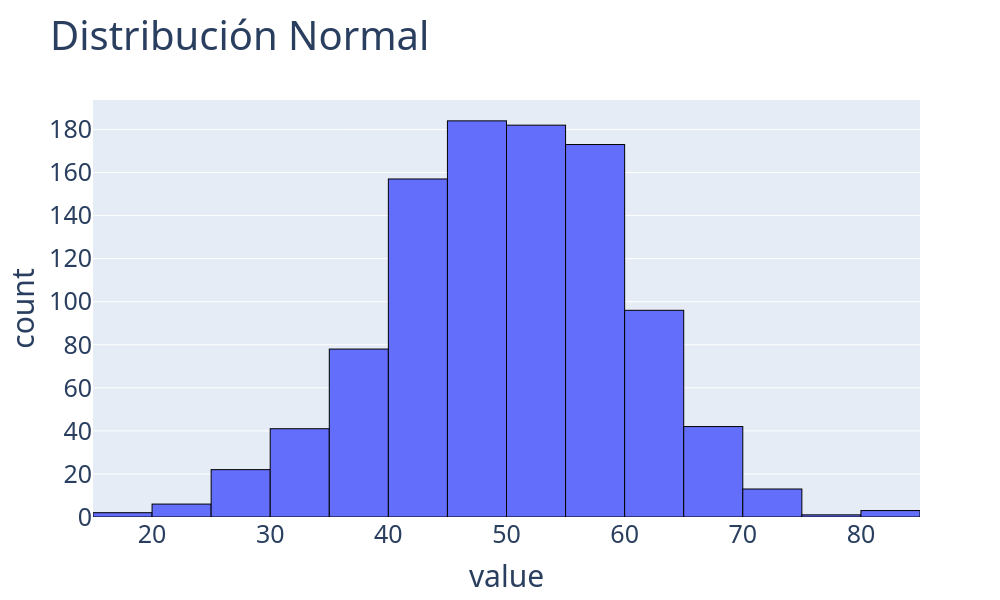
\includegraphics[width=\textwidth]{imgs/plots/histplot_01.png}
                \end{figure}
            \column{0.5\textwidth}%\pause
                \begin{figure}
                \centering
                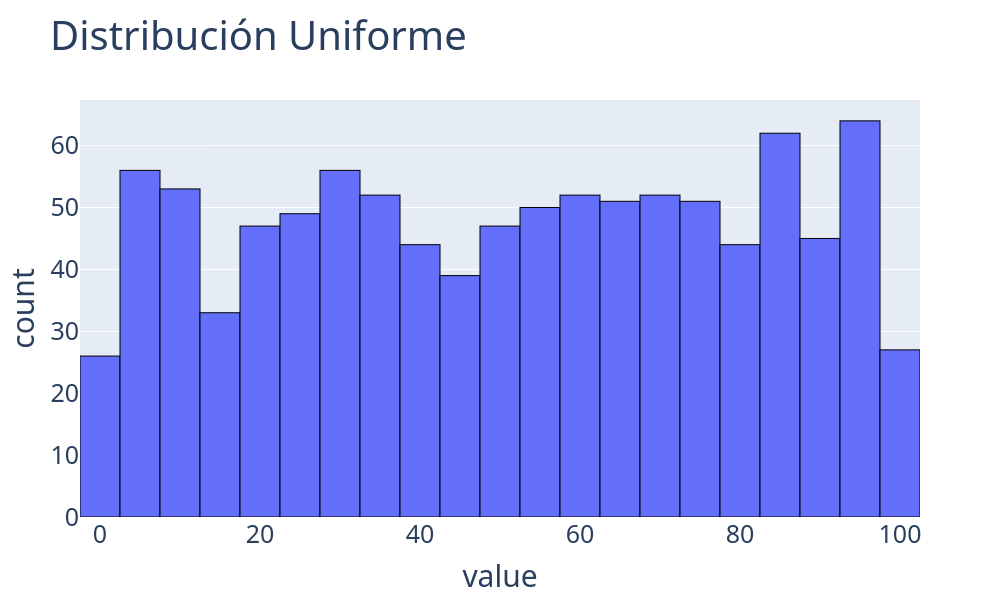
\includegraphics[width=\textwidth]{imgs/plots/histplot_02.png}
                \end{figure}
        \end{columns}
    \end{frame}

    \begin{frame}{II.II~$\rhd$~Estadística Descriptiva - Visualización: Histograma}
        \begin{columns}
            \column{0.48\textwidth}
            \begin{figure}
                \centering
                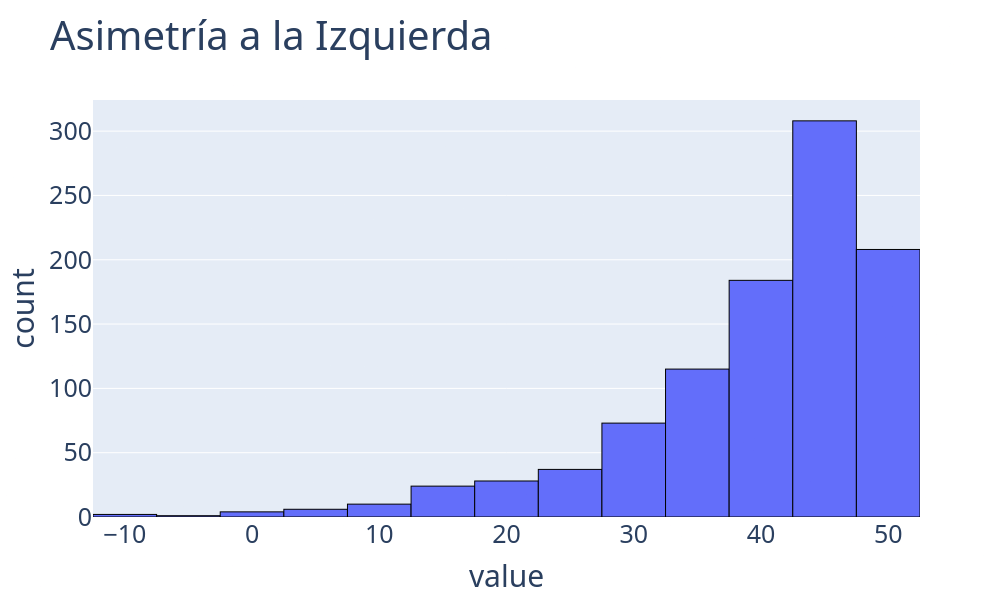
\includegraphics[width=\textwidth]{imgs/plots/histplot_03.png}
            \end{figure}
            \column{0.48\textwidth}%\pause
            \begin{figure}
                \centering
                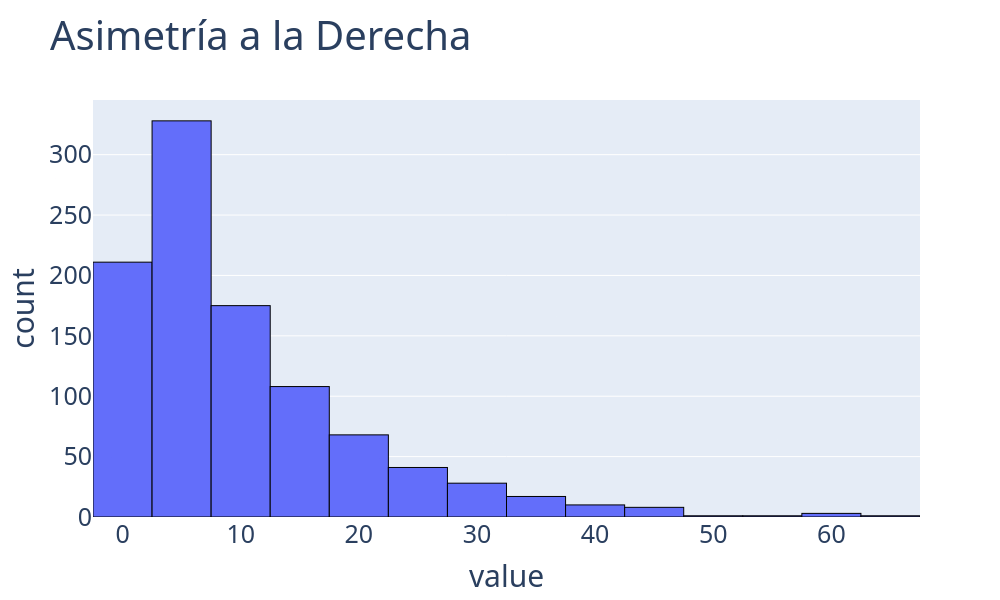
\includegraphics[width=\textwidth]{imgs/plots/histplot_04.png}
            \end{figure}
        \end{columns}
        % \vspace{3mm}
        \begin{columns}
            \column{0.48\textwidth}%\pause
            \begin{figure}
                \centering
                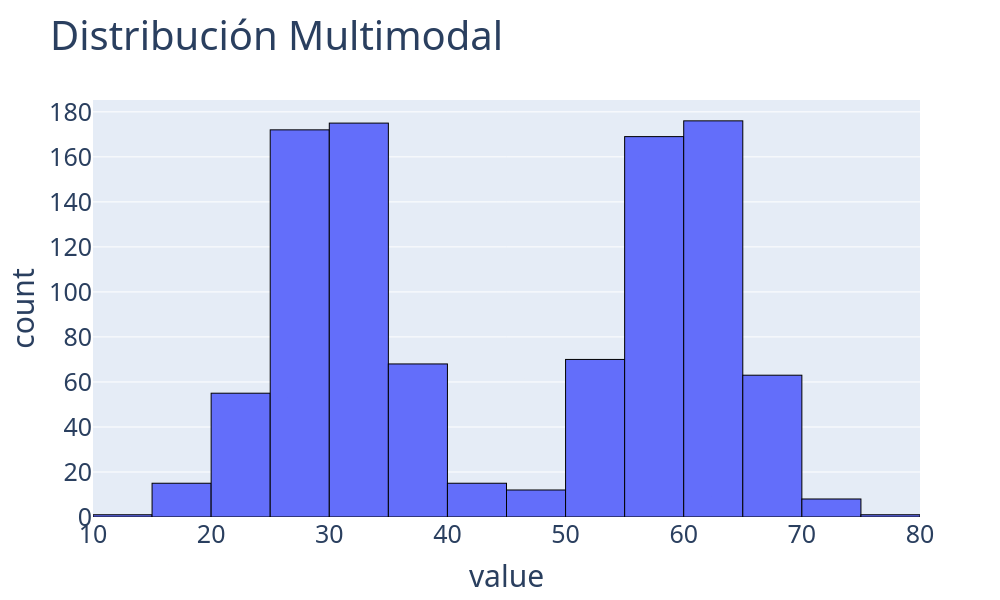
\includegraphics[width=\textwidth]{imgs/plots/histplot_05.png}
            \end{figure}
        \end{columns}
    \end{frame}

    \begin{frame}{II.II~$\rhd$~Estadística Descriptiva - Visualización: Boxplot}
        \begin{itemize}
            \item Representa la \textcolor{DarkOrchid}{tendencia central} y la \textcolor{DarkOrchid}{dispersión} del conjunto de datos.
            \vspace{2mm}%\pause
            \item Considera los cuartiles: $Q_{1}$ (percentil 25), $Q_{2}$ (percentil 50, mediana) y $Q_{3}$ (percentil 75), además de los valores máximo y mínimo.
            \vspace{2mm}%\pause
            \item Permite identificar \textcolor{DarkOrchid}{valores atípicos (outliers)} que se encuentran más allá de la \textit{bulk data} (zona central de los datos).
        \end{itemize}
        \vspace{5mm}%\pause
        \begin{figure}
            \centering
            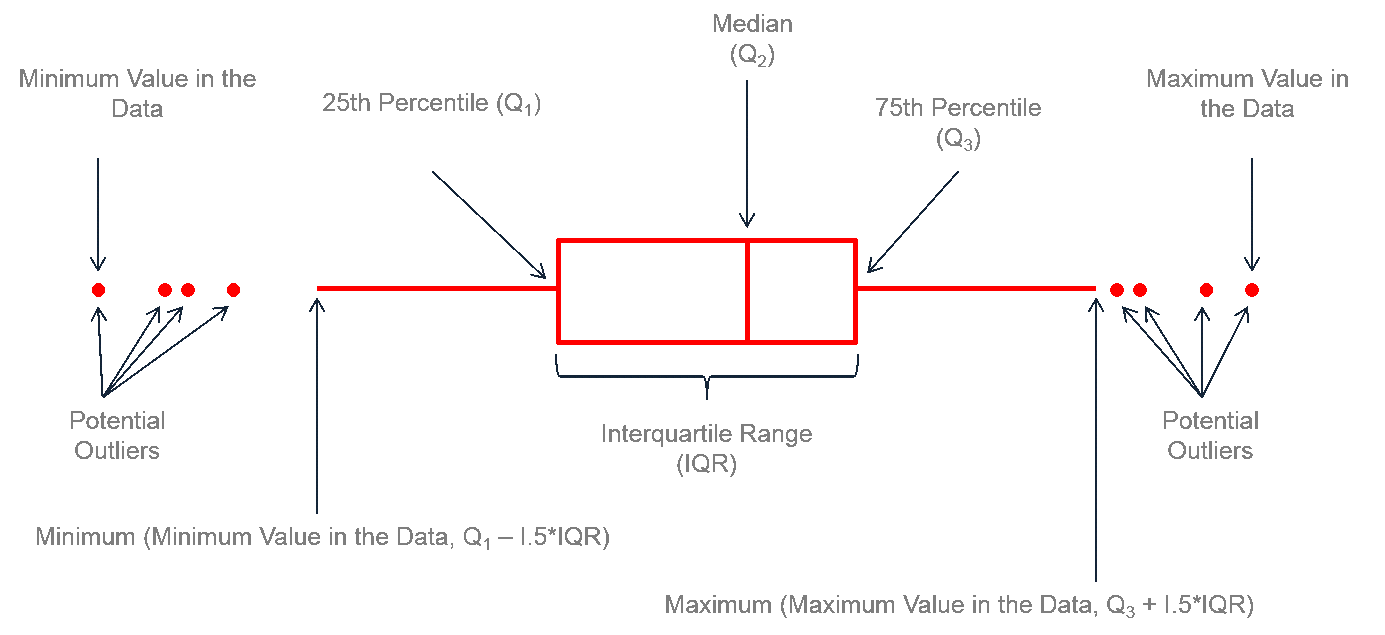
\includegraphics[width=0.8\textwidth]{imgs/t1_img4.png}
        \end{figure}
    \end{frame}

    \begin{frame}{II.II~$\rhd$~Estadística Descriptiva - Visualización: Violin Plots}
        \begin{figure}
            \centering
            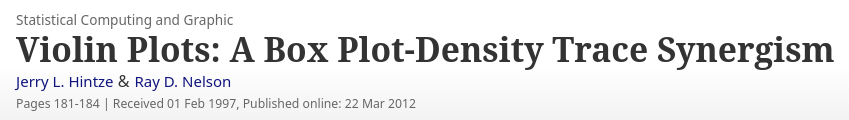
\includegraphics[width=\textwidth]{imgs/violin/title.png}
        \end{figure}%\pause
        \begin{itemize}
            \item Combina un \textcolor{DarkOrchid}{Boxplot} con una \textcolor{DarkOrchid}{traza de densidad}~(métodos de \textit{smoothed histogram} como KDE).
        \end{itemize}%\pause
        \begin{columns}
            \column{0.5\textwidth}
                \begin{figure}
                \centering
                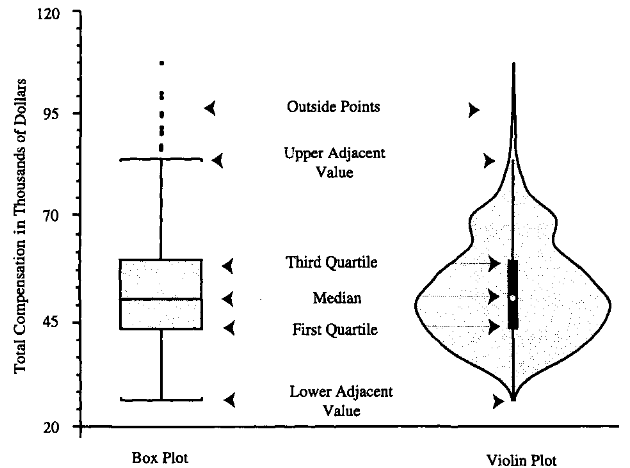
\includegraphics[width=0.9\textwidth]{imgs/violin/plot_01.png}
                \end{figure}
            \column{0.5\textwidth}
                \begin{itemize}
                    \item Boxplot:%\pause (I) la linea de la media se cambia por un punto,%\pause (II) los outliers no se identifican individualmente como marcas.%\pause
                    \item Traza de Densidad:%\pause Muestra la distribución características de los datos por medio de un estimador de densidad.
                \end{itemize}
        \end{columns}
    \end{frame}

    \begin{frame}{II.II~$\rhd$~Estadística Descriptiva - Visualización: Violin Plots}
        \begin{exampleblock}{Ejemplo 1}
        Consideremos dos clusters con las siguiente distribución respectivamente: $\text{Cluster 1} \sim \mathcal{N}(\boldsymbol{\mu}_1=30, \Sigma=3)$ y $\text{Cluster 2} \sim \mathcal{N}(\boldsymbol{\mu}_2=60, \Sigma=3)$.
        \end{exampleblock}
        %\pause
        \begin{figure}
            \centering
            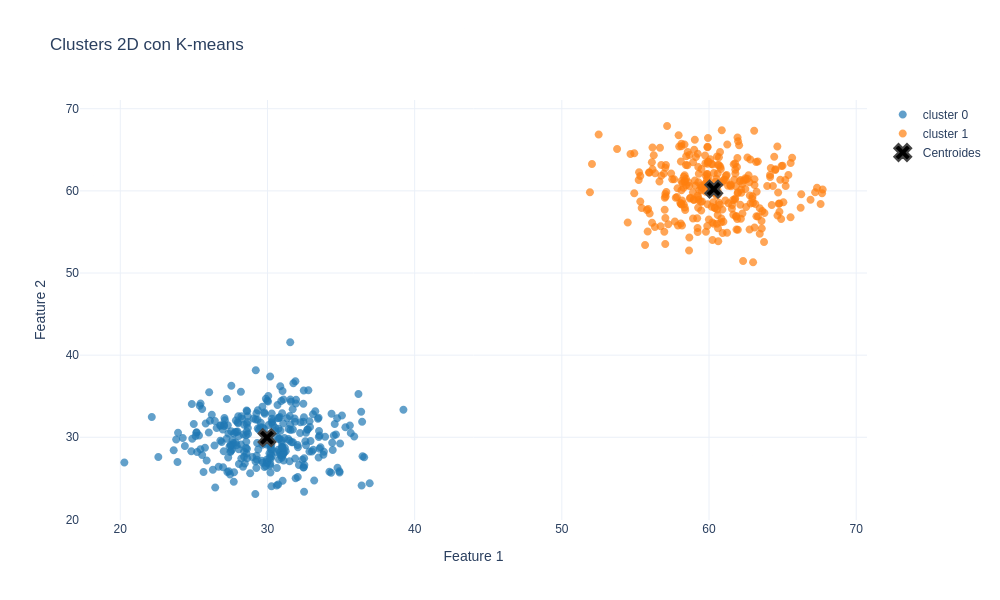
\includegraphics[width=0.8\textwidth]{imgs/violin/ej_01.png}
        \end{figure}
    \end{frame}

    \begin{frame}{II.II~$\rhd$~Estadística Descriptiva - Visualización: Violin Plots}
        \begin{exampleblock}{Ejemplo 1}
        Consideremos dos clusters con las siguiente distribución respectivamente: $\text{Cluster 1} \sim \mathcal{N}(\boldsymbol{\mu}_1=30, \Sigma=3)$ y $\text{Cluster 2} \sim \mathcal{N}(\boldsymbol{\mu}_2=60, \Sigma=3)$.
        \end{exampleblock}
        \begin{figure}
            \centering
            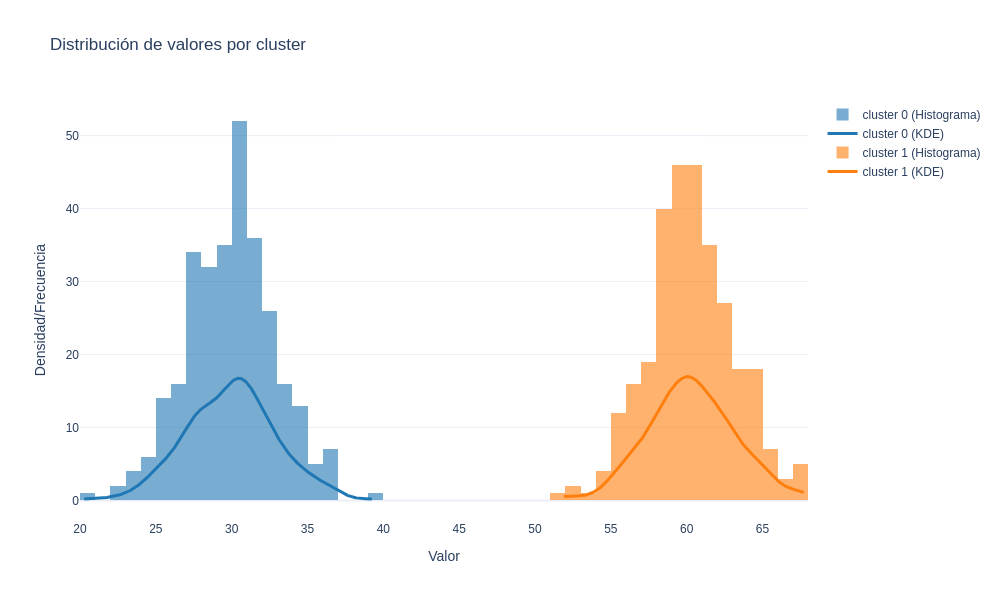
\includegraphics[width=0.8\textwidth]{imgs/violin/ej_02.png}
        \end{figure}
    \end{frame}

    \begin{frame}{II.II~$\rhd$~Estadística Descriptiva - Visualización: Violin Plots}
        \begin{exampleblock}{Ejemplo 1}
        Consideremos dos clusters con las siguiente distribución respectivamente: $\text{Cluster 1} \sim \mathcal{N}(\boldsymbol{\mu}_1=30, \Sigma=3)$ y $\text{Cluster 2} \sim \mathcal{N}(\boldsymbol{\mu}_2=60, \Sigma=3)$.
        \end{exampleblock}
        \begin{figure}
            \centering
            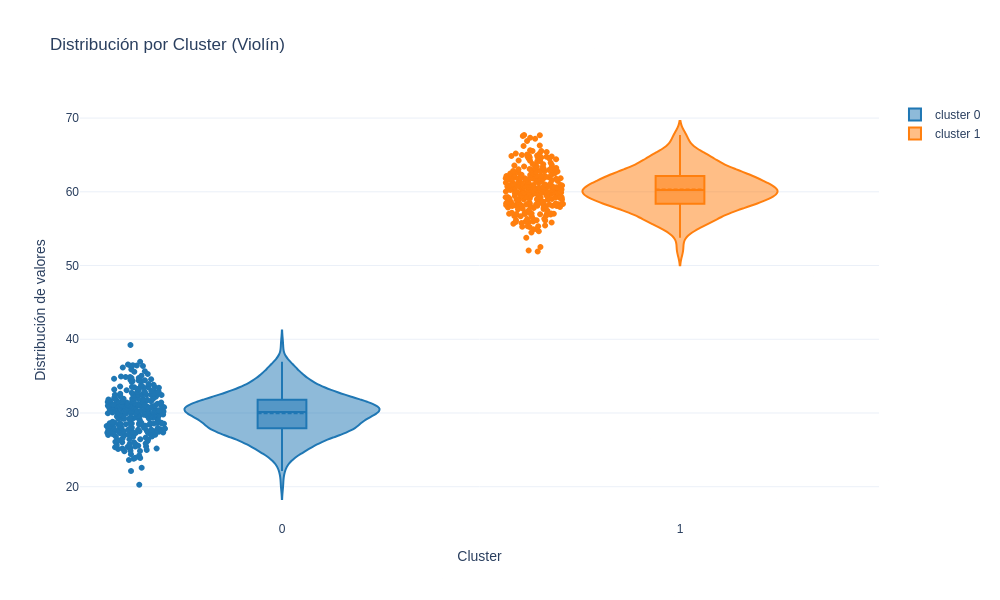
\includegraphics[width=0.8\textwidth]{imgs/violin/ej_03.png}
        \end{figure}
    \end{frame}

    \begin{frame}{II.II~$\rhd$~Estadística Descriptiva - Visualización: Violin Plots}
        \textbf{¿Qué diferencias hay con un Boxplot?}
        \vspace{5mm}
        \begin{itemize}
            \item Entrega un mejor entendimiento respecto a la forma de la distribución de los datos.%\pause
            \item Muestra la existencias de clústeres.
            \item Resalta los peaks, valles y bumps de la distribución.
        \end{itemize}
        \vspace{5mm}%\pause
        \begin{exampleblock}{Ejemplo 2}
        Consideremos los siguientes tres samples de $10.000$ elementos cada uno:
        \begin{itemize}
            \item Sample 1 $\sim \mathcal{N}(\boldsymbol{\mu}=30, \Sigma=5) + \mathcal{N}(\boldsymbol{\mu}=60, \Sigma=5)$
            \item Sample 2 $\sim \mathcal{N}(\boldsymbol{\mu}=50, \Sigma=5)$
            \item Sample 3 $\sim \mathcal{U}(\text{min}=20, \text{max}=60)$
        \end{itemize}
        \end{exampleblock}
    \end{frame}

    \begin{frame}{II.II~$\rhd$~Estadística Descriptiva - Visualización: Violin Plots}
        \begin{figure}
        \centering
        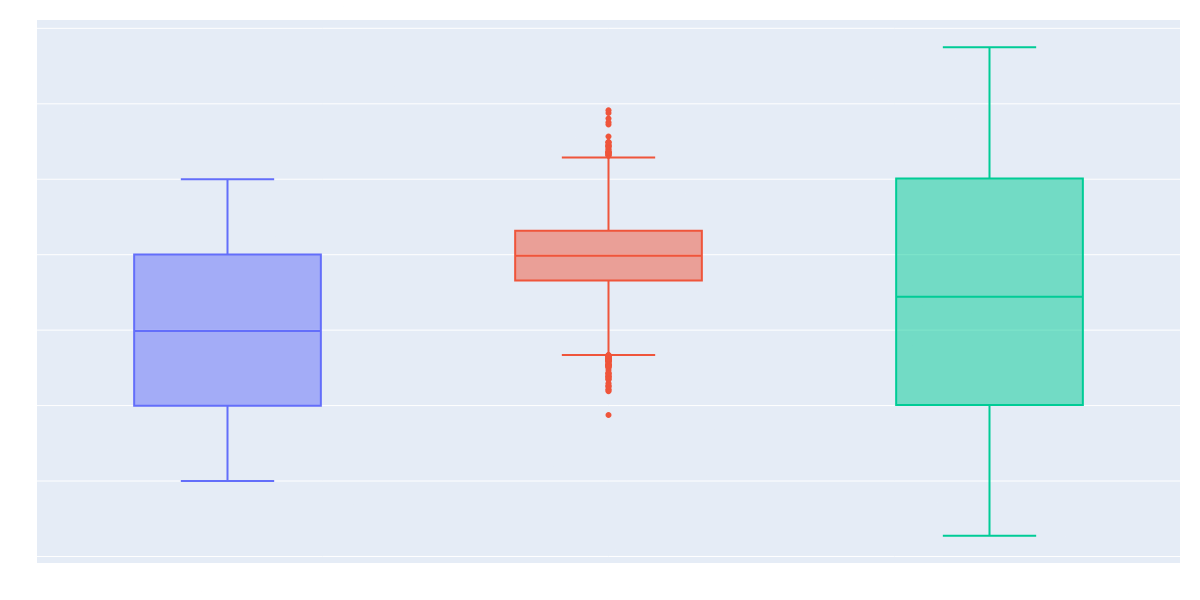
\includegraphics[width=\textwidth]{imgs/violin/ej2_01.png}
        \end{figure}
    \end{frame}

    \begin{frame}{II.II~$\rhd$~Estadística Descriptiva - Visualización: Violin Plots}
        \begin{figure}
        \centering
        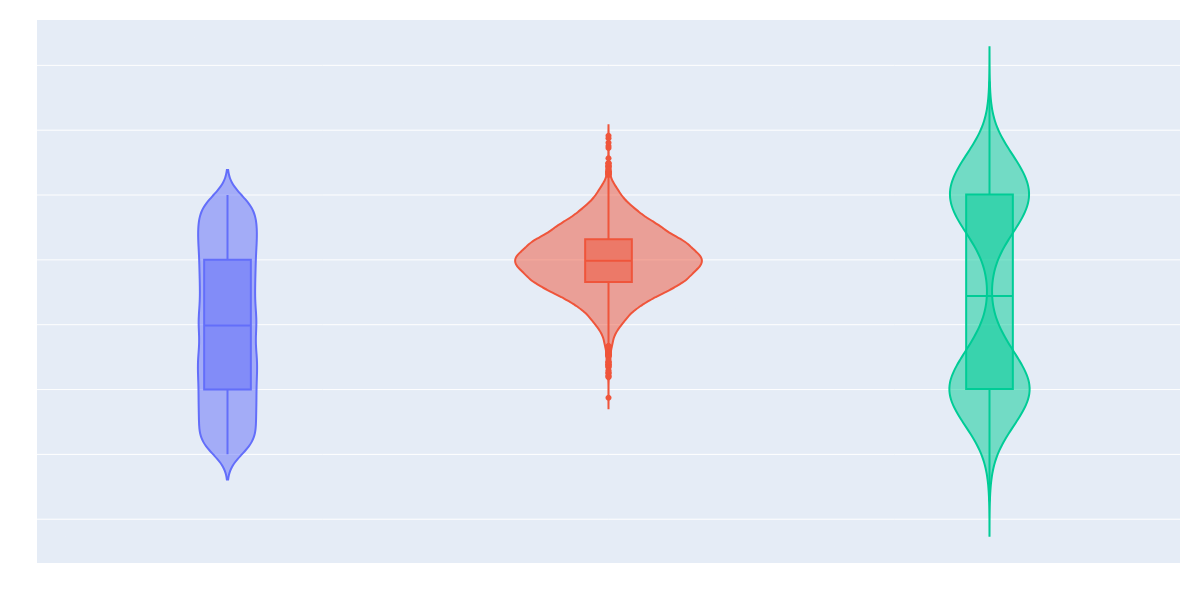
\includegraphics[width=\textwidth]{imgs/violin/ej2_02.png}
        \end{figure}
    \end{frame}

    \begin{frame}{II.II~$\rhd$~Estadística Descriptiva - Visualización: Violin Plots}
        \begin{figure}
        \centering
        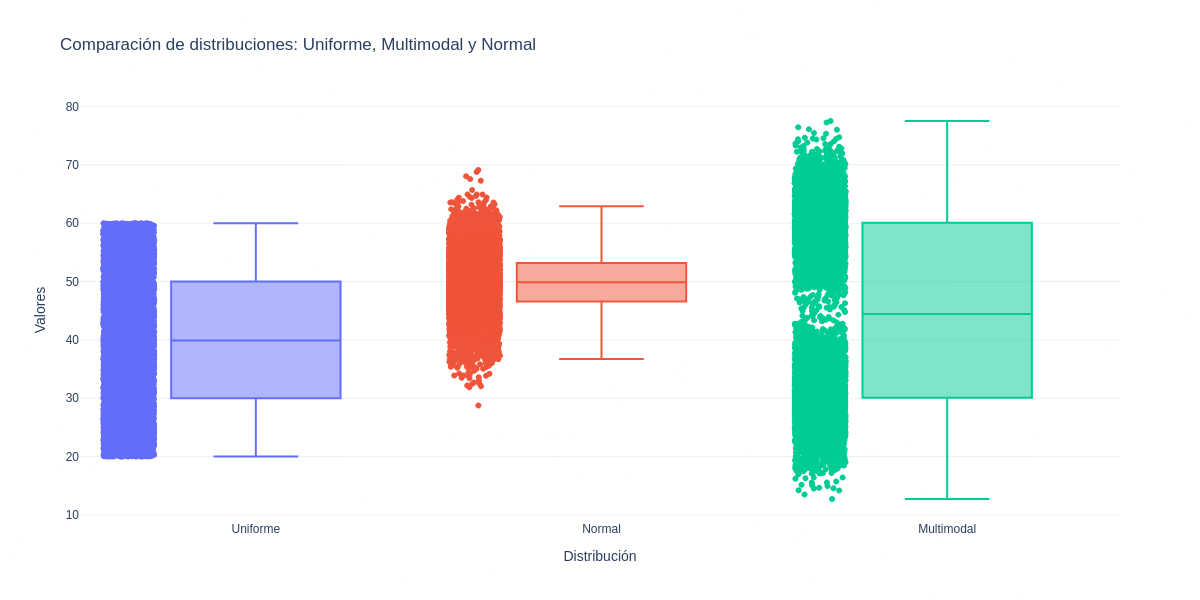
\includegraphics[width=\textwidth]{imgs/violin/ej2_03.png}
        \end{figure}
    \end{frame}

    \begin{frame}{II.II~$\rhd$~Estadística Descriptiva - Visualización: Violin Plots}
        \begin{figure}
        \centering
        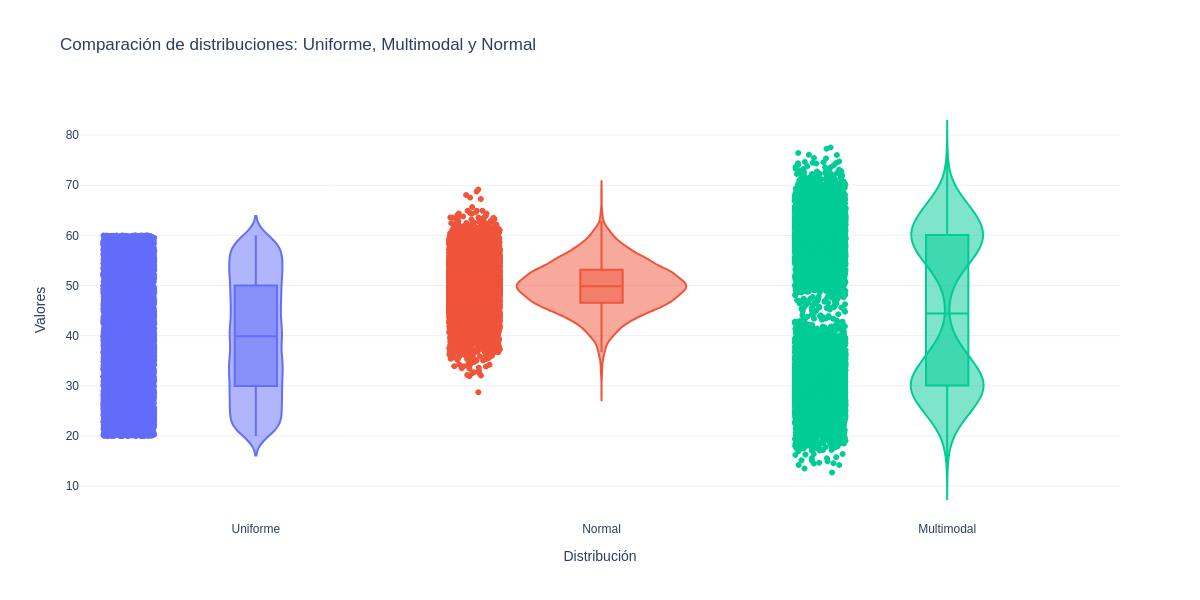
\includegraphics[width=\textwidth]{imgs/violin/ej2_04.png}
        \end{figure}
    \end{frame}

    \section{Pre-Procesamiento de Datos}
    \begin{frame}{III~$\rhd$~ Calidad de los Datos} 
        \begin{block}{¿Por qué es importante la calidad de los datos?}
            \begin{itemize}
                \item Buscamos que nuestros datos tengan las siguientes características:
                \begin{itemize}
                    \item \textbf{Precisión} (Accuracy)
                    \item \textbf{Completitud} (Completeness)
                    \item \textbf{Consistencia} (Consistency)
                \end{itemize}
                \vspace{5mm}%\pause
                \item Los pasos más comunes para el preprocesamiento son:
                \begin{itemize}
                    \item \textbf{Data Cleaning}: Manejo de valores faltantes, ruido y outliers
                    \item \textbf{Data Integration}: Combinación de múltiples fuentes
                \end{itemize}
            \end{itemize}
        \end{block}
    \end{frame}

    \begin{frame}{III.I~$\rhd$~ Data Cleaning}
        \begin{itemize}
            \item La limpieza de los datos busca corregir datos faltantes, suavizar el ruido en los datos, o simplemente identificar o remover inconsistencias como los outliers.
            \vspace{5mm}%\pause
            \item Consideremos los siguientes escenarios clásicos:
            \begin{enumerate}
                \item Noisy Data
                \item Missing Values
            \end{enumerate}
        \end{itemize}
    \end{frame}

    \begin{frame}{III.I~$\rhd$~ Data Cleaning - Noisy Data}
        \begin{itemize}
            \item El ruido en los datos (\textit{noise}) es un error aleatorio dentro de estos.
            \item Las Visualizaciones de estadística descriptiva suelen identificarlo, por ejemplo en los boxplot o violin plots.
            \item Para eliminarlo, debes \textit{'suavizar'} los datos (smoothing process).
            \vspace{4mm}%\pause
            \item La técnica mas popular de suavizamiento es \textbf{Binning}:
            \begin{itemize}
                \item Dividir los \textbf{datos ordenados} en 'bins' (o 'buckets')
                \item Reemplazar los valores originales dentro de cada bin por un valor representativo
                \item Los reemplazos pueden ser utilizando: media (smoothing by bin means), mediana (smoothing by bin medians), min-max ((smoothing by bin boundaries).
            \end{itemize}
        \end{itemize}
    \end{frame}

    \begin{frame}{III.I~$\rhd$~ Data Cleaning - Noisy Data}
        \begin{exampleblock}{Ejemplo 3 - Binning}
        Consideremos la siguiente distribución de datos:
        \lstinputlisting[language=Python, basicstyle=\tiny]{codes/ej5.py}
        \end{exampleblock}
    \end{frame}

    \begin{frame}{III.I~$\rhd$~ Data Cleaning - Noisy Data}
        \begin{figure}
            \centering
            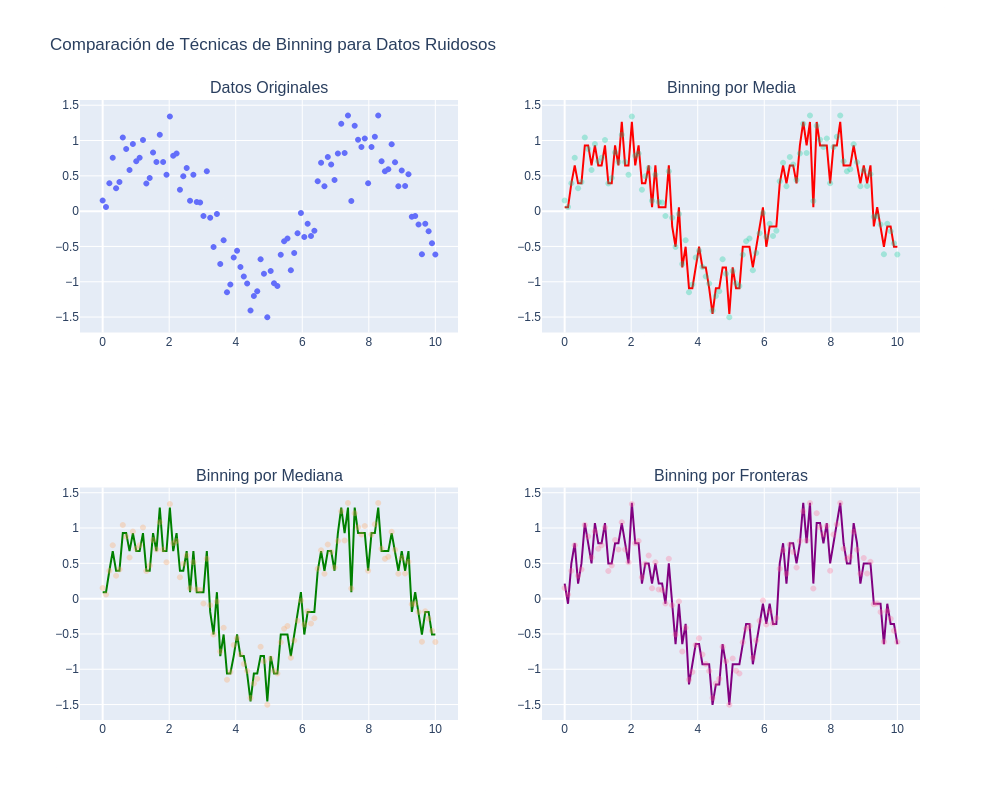
\includegraphics[width=0.8\linewidth]{imgs/noise/ej1.png}
        \end{figure}
    \end{frame}

    \begin{frame}{III.I~$\rhd$~ Data Cleaning - Noisy Data}
        \begin{figure}
            \centering
            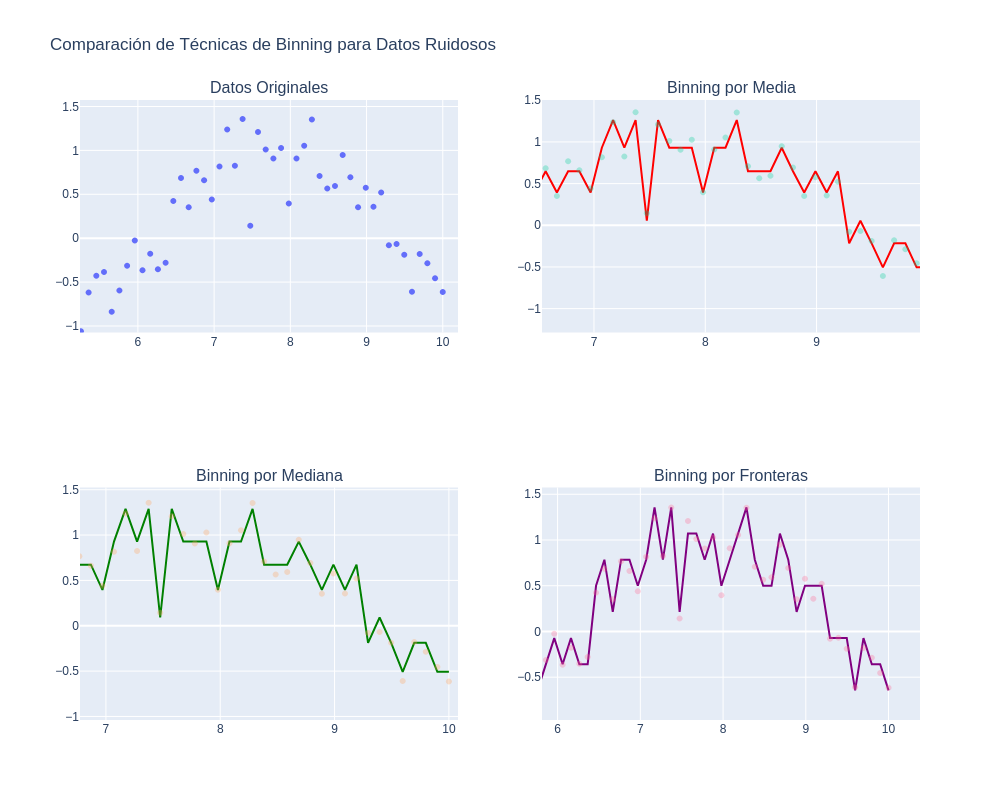
\includegraphics[width=0.8\linewidth]{imgs/noise/ej2.png}
        \end{figure}
    \end{frame}

    \begin{frame}[fragile]{III.I~$\rhd$~ Data Cleaning - Missing Values}
        \begin{exampleblock}{Ejemplo 4}
        \lstinputlisting[language=Python, basicstyle=\tiny]{codes/ej1.py}
        \end{exampleblock}
        \vspace{3mm}
        \begin{itemize}
            \item Los \textit{missing values} suelen verse reflejada en aquellos valores \texttt{None} o \texttt{np.nan} que vemos en los datsets.
            \item \textbf{Importante !} No siempre los \textit{missing values} implican un error ~$\rightarrow$~ e.g. Preguntas opcionales en encuestas.
        \end{itemize}
    \end{frame}

    \begin{frame}[fragile]{III.I~$\rhd$~ Data Cleaning - Missing Values}
        \textbf{¿Que alternativas tenemos?}
        \vspace{3mm}
        \begin{itemize}
            \item Ignorar los registros con \textit{missing values}. No es efectivo, a menos que el feature tengo demasiados missing values.
            %\pause
            \item Rellenar los valores faltantes de manera manual. Costoso en tiempo y recursos.
            %\pause
            \begin{itemize}
                \item Usar una constante para identificar los \textit{missing values}, como \texttt{'Missing'}, \texttt{-1}, \texttt{0}, \texttt{'Unknown'}~$\rightarrow$~No siempre es 'foolproof'.
            \end{itemize}
            \vspace{3mm}%\pause
            \item Imputación de valores:
            \begin{itemize}
                \item Usar una medida de tendencia central, como \textit{Mean Imputation} o \textit{Median Imputation}. Para datos distribuidos normalmente (simétricos), usar la media. Para datos asimétricos (skewed data), usar la mediana.
                %\pause
                \item Usar los \textit{'valores más probables'}. Por medio de una regresión, o usando inferencia bayesiana.
            \end{itemize}
        \end{itemize}
    \end{frame}

    \begin{frame}[fragile]{III.I~$\rhd$~ Data Cleaning - Missing Values}
        \textbf{Imputación de valores}
        \vspace{3mm}
        \begin{itemize}
            \item Problema: Inyección de sesgo estadístico en los datos (Data Bias).
            %\pause
            \item Alternativas actuales~$\rightarrow$~\textbf{k-Nearest Neighbors Imputation}: los missing values son imputados por valores más cercanos de acuerdo a una métrica de \textit{similaridad} respecto a patrones en el dataset.
        \end{itemize}
        %\pause
        \begin{exampleblock}{Ejemplo 5 - \texttt{sklearn.impute.SimpleImputer} - Mean - Axis 0}
        \lstinputlisting[language=Python, basicstyle=\tiny]{codes/ej2.py}
        \end{exampleblock}
    \end{frame}

    \begin{frame}[fragile]{III.I~$\rhd$~ Data Cleaning - Missing Values}
        \begin{exampleblock}{Ejemplo 6 - \texttt{sklearn.impute.SimpleImputer} - Median - Axis 0}
        \lstinputlisting[language=Python, basicstyle=\tiny]{codes/ej3.py}
        \end{exampleblock}
    \end{frame}

    \begin{frame}[fragile]{III.I~$\rhd$~ Data Cleaning - Missing Values}
        \begin{exampleblock}{Ejemplo 7 - \texttt{sklearn.impute.KNNImputer} - k=2 - Axis 0}
        \begin{columns}
            \column{0.7\textwidth}
                \begin{figure}
                \centering
                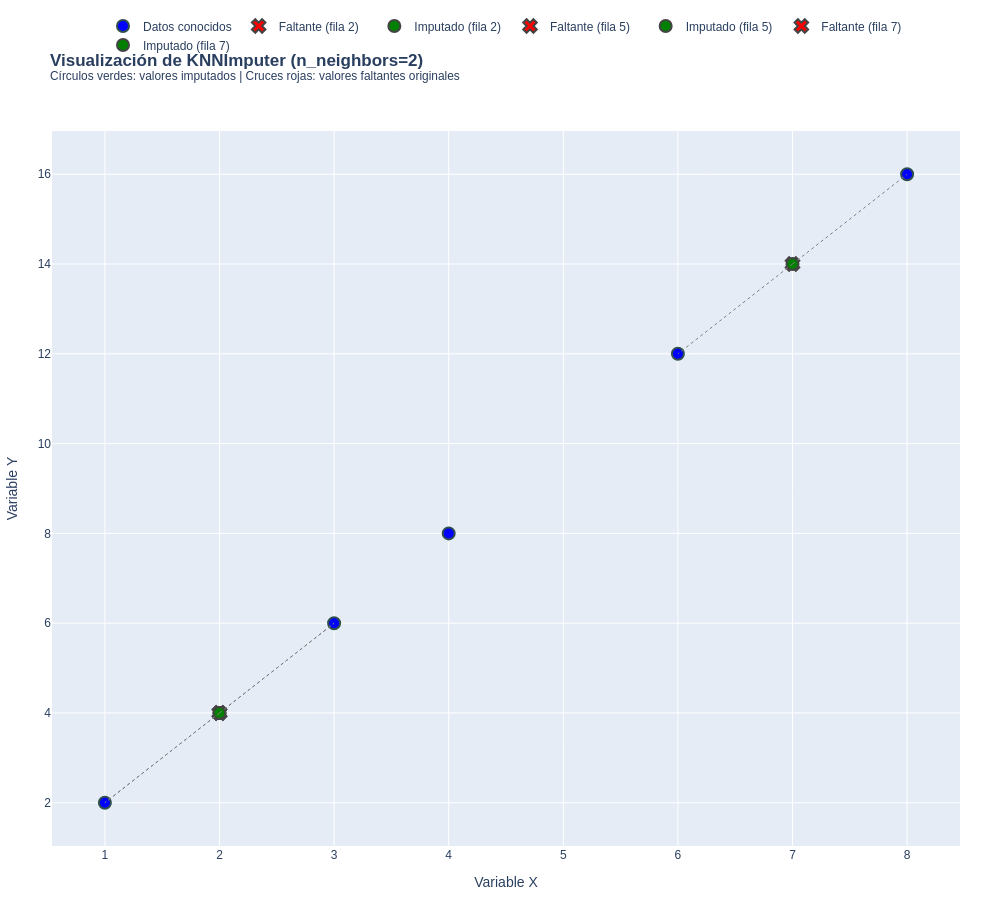
\includegraphics[width=0.8\textwidth]{imgs/imp/ej1.png}
                \end{figure}
            \column{0.3\textwidth}
                \lstinputlisting[language=Python, basicstyle=\tiny]{codes/ej4.py}
        \end{columns}
        \end{exampleblock}
    \end{frame}

    \begin{frame}{III.II~$\rhd$~ Data Integration}
        \begin{itemize}
            \item Caso típico: fusión de múltiples fuentes de datos en un único conjunto.
            \vspace{4mm}%\pause
            \item Problemas frecuentes en la integración:
            \begin{itemize}
                \item \textbf{Redundancia}: Ocurre cuando un dato puede derivarse de otros atributos.
                \item \textbf{Inconsistencia}: Puede surgir como consecuencia de redundancias en los datos.
            \end{itemize}
            \vspace{4mm}%\pause
            \item Detección de redundancias mediante \textbf{análisis de correlación}:
            \begin{itemize}
                \item \textbf{Test de correlación~$\chi^{2}$}: Para variables nominales/categóricas.
                \item \textbf{Coeficiente de correlación} y \textbf{covarianza}: Para variables numéricas.
            \end{itemize}
        \end{itemize}
    \end{frame}

    \begin{frame}{III.II~$\rhd$~ Data Integration - Test de correlación~$\chi^{2}$}
    \scriptsize{
    % \framesubtitle{Test de correlación~$\chi^{2}$}
        \begin{itemize}
            \item Supongamos que buscamos la correlación entre dos atributos $A$ y $B$, nominales, de un dataset.
            %\pause
            \item $A$ tiene $c$ valores distintos $a_{1},a_{2},...,a_{c}$, mientras que $B$ tiene $r$ valores distintos $b_{1},b_{2},...,b_{r}$.
            %\pause
            \item Definimos la \textbf{tabla de contingencia} como la matriz de $c$ columnas y $r$ filas, tal que $(A_{i}, B_{j})$ denote \textbf{frecuencia observada combinada} de que el atributo $a_{i}$ de $A$ tome el valor de ocurrencia del atributo $b_{j}$ de $B$.
        \end{itemize}
        %\pause
        \begin{block}{Definición}
        Dada una tabla de contingencia con $r$ filas y $c$ columnas, el valor del test de correlación~$\chi^{2}$ es:
        \[
        \chi^2 = \sum_{i=1}^{c}\sum_{j=1}^{r} \frac{(o_{ij} - e_{ij})^2}{e_{ij}}
        \]
        donde:
        \begin{itemize}
            \item $o_{ij}$ = Valor observado en la celda $(i,j)$, \textbf{frecuencia observada} del evento $(A_{i}, B_{j})$.
            \item $e_{ij} = \frac{\text{Total fila }i \times \text{Total columna }j}{\text{Gran total}}$ y es la \textit{frecuencia esperada} del evento $(A_{i}, B_{j})$. 
            \item Grados de libertad: $(r-1)(c-1)$
        \end{itemize}
        \end{block}
    }
    \end{frame}
    % Los valores esperados en una tabla de contingencia (usada en el test chi-squere) representan las frecuencias teóricas que se esperarían si no hubiera asociación entre las variables analizadas (es decir, si fueran independientes). Se calculan bajo la hipótesis nula (H0) de que no existe relación entre las variables.

    \begin{frame}{III.II~$\rhd$~ Data Integration - Test de correlación~$\chi^{2}$}
        \scriptsize{\textcolor{DarkOrchid}{El Test de correlación~$\chi^{2}$ tiene por hipótesis que $A$ y $B$ son \textbf{independientes}, osea que no están correlacionados entre ellos.}}
        %\pause
        \begin{exampleblock}{Ejemplo 8 - \texttt{scipy.stats. chi2\_contingency}}
            \lstinputlisting[basicstyle=\tiny]{codes/ej6_1.py}
            %\pause
            \lstinputlisting[basicstyle=\tiny]{codes/ej6_2.py}
            %\pause
            \lstinputlisting[basicstyle=\tiny]{codes/ej6_3.py}
        \end{exampleblock}
    \end{frame}

    \begin{frame}{III.II~$\rhd$~ Data Integration - Covarianza}
    \scriptsize{
        %\pause
        \begin{itemize}
            \item Buscamos evaluar cómo varían conjuntamente dos atributos numéricos $A$ y $B$ respecto a sus \textbf{medias}.
        \end{itemize}
        %\pause
        \begin{block}{Definición}
            Dadas dos variables numéricas \( A \) y \( B \), con \( n \) observaciones cada una, la \textbf{covarianza} se define como:
            \[
            \text{Cov}(A, B) = \frac{1}{n} \sum_{i=1}^{n} (A_i - \bar{A})(B_i - \bar{B})
            \]
        
            \begin{itemize}
                \item \( A_i \) y \( B_i \): Valores individuales de las variables \( A \) y \( B \).
                \item \( \bar{A} \) y \( \bar{B} \): Medias muestrales de \( A \) y \( B \), respectivamente.
                \item \( n \): Número de observaciones.
            \end{itemize}
        \end{block}
        %\pause
        \begin{itemize}
            \item Covarianza \( > 0 \): Relación directa (ambas variables tienden a aumentar o disminuir juntas).
            \item Covarianza \( < 0 \): Relación inversa (una aumenta mientras la otra disminuye).
            \item Covarianza \( = 0 \): No hay relación lineal (puede haber independencia o una relación no lineal).
        \end{itemize}
    }
    \end{frame}

    \begin{frame}{III.II~$\rhd$~ Data Integration - Covarianza}
        \begin{figure}
            \centering
            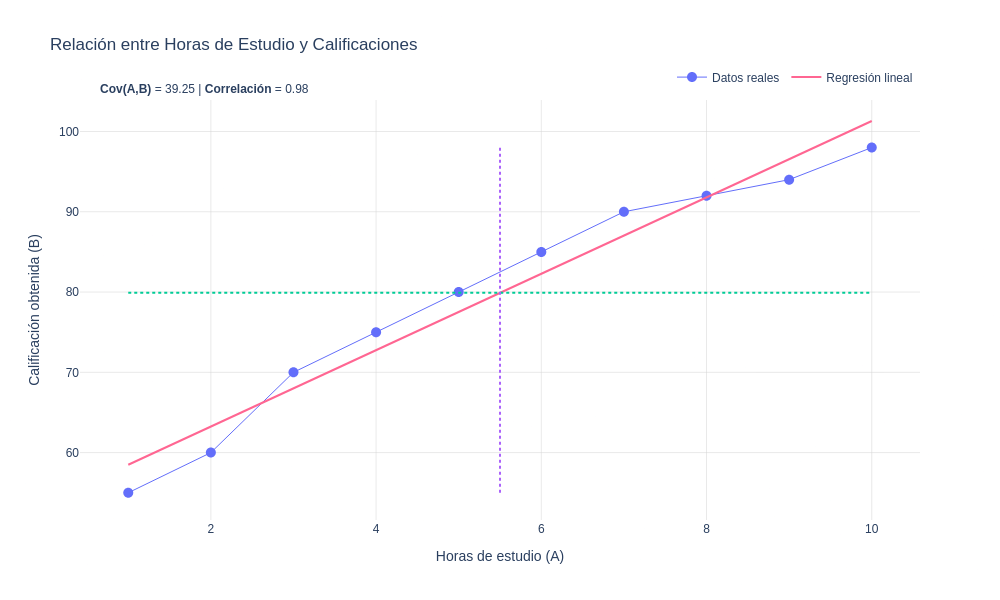
\includegraphics[width=\linewidth]{imgs/corr/ej2.png}
        \end{figure}
    \end{frame}

    \begin{frame}{III.II~$\rhd$~ Data Integration - Coeficiente de Correlación}
        %\pause
        \begin{itemize}
            \item Conocido como \textit{Pearson correlation coefficient} o \textit{Pearson's product moment coefficient}.
            %\pause
            \item Buscamos evaluar la correlación entres dos atributos numéricos $A$ y $B$ de un dataset.
        \end{itemize}
        %\pause
        \begin{block}{Definición}
            El coeficiente de correlación $r_{AB}$ se define como:
            \[
            r_{AB} = \frac{\text{Cov}(A,B)}{\sigma_A \sigma_B} = \frac{\sum_{i=1}^n (A_i - \bar{A})(B_i - \bar{B})}{\sqrt{\sum_{i=1}^n (A_i - \bar{A})^2} \sqrt{\sum_{i=1}^n (B_i - \bar{B})^2}}
            \]
            donde:
            \begin{itemize}
            \item $\bar{A}$ y $\bar{B}$ son las medias muestrales
            \item $\text{Cov}(A,B)$ es la covarianza entre $A$ y $B$
            \item $\sigma_A$, $\sigma_B$ son las desviaciones estándar
            \end{itemize}
        \end{block}
    \end{frame}

    \begin{frame}{III.II~$\rhd$~ Data Integration - Coeficiente de Correlación}
        \begin{alertblock}{Propiedades}
            \begin{itemize}
            \item $-1 \leq r_{AB} \leq 1$
            \item $r_{AB} = 1$: Correlación lineal positiva perfecta
            \item $r_{AB} = -1$: Correlación lineal negativa perfecta
            \item $r_{AB} = 0$: No hay correlación lineal
            \end{itemize}
        \end{alertblock}
        \vspace{5mm}
        %\pause
        \begin{exampleblock}{Ejemplo 9}
            \lstinputlisting[language=Python, basicstyle=\scriptsize]{codes/ej7.py}
        \end{exampleblock}
    \end{frame}

    \begin{frame}{III.II~$\rhd$~ Data Integration - Coeficiente de Correlación}
        \scriptsize{\textcolor{DarkOrchid}{El Coeficiente de Correlación tiene por hipótesis que $A$ y $B$ son \textbf{independientes}, osea que \textbf{no} están correlacionados entre ellos.}}\footnote{\scriptsize{Rechazamos con $p-value<0.05$.}}
        \vspace{3mm}
        \begin{figure}
            \centering
            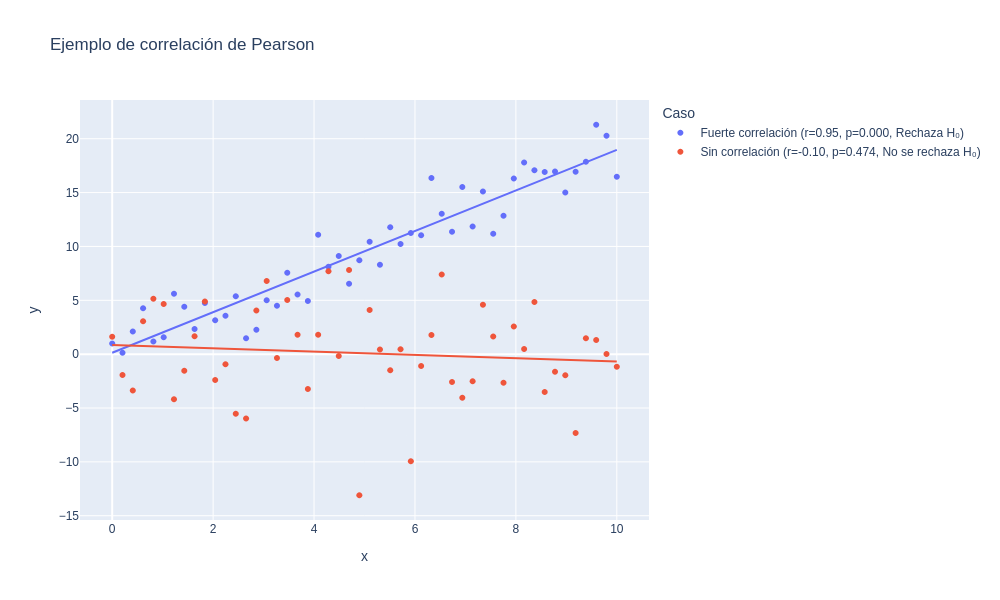
\includegraphics[width=0.9\linewidth]{imgs/corr/ej1.png}
        \end{figure}
    \end{frame}
\end{document}